\setcounter{page}{1}
\setcounter{figure}{0}  % reset counter

\section{Supplemental results for the Simulated dataset} \label{sec:simulation}
%\begin{enumerate}
%\item Why to do simulation?
%\item How to generate simulation data?
%\item Statistics. \\
%How many simulated systems, how many variants are present, how many valid sites.\\
%Distribution of number of groups, valid groups, and valid variants per group?
%\item Do we identify the present variants correctly?
%\item Do we accurately quantify the present variants?
%\item What is the FDR for variant group identification?
%\end{enumerate}

We apply our framework on simulated data to test how well we are able to identify the present modification variants and recover their actual relative abundances from a mixture MS/MS spectrum. We generate simulated data based on the $209$ unique unmodified peptides which were identified from the lens dataset by at least two spectra. For each unmodified peptide, we create mixture spectra of its variants which are singly modified with $+43$. We allow the modification to occur on only valid sites (N terminal *, R, K) to account for also the distribution of the number and position of the sites in real data. The distribution of the number of valid sites of $+43$ for our set of peptide sequences are shown in Table~\ref{tbl:SimDistNumValidSites}.

\begin{table}[h]
\centering
\caption{Number of valid sites of +43 in the set of peptide sequences chosen for simulation.}
\label{tbl:SimDistNumValidSites}
\begin{tabular}{|l|l|}
\hline
\#valid sites & \#cases\\
\hline
$\ge 1$ & 209 \\
\hline
$\ge 2$ & 205 \\
\hline
$\ge 3$ & 58 \\
\hline
$== 4$ & 4 \\
\hline
\end{tabular}
\end{table}

Each simulated dataset consists of an unmodified peptide sequence, an unmodified spectrum to be used for inference of detectabilities, and a mixture spectrum. Given unmodified peptide $p$, we generate $100$ different such datasets of $k \leq 3$ co-eluting peptide variants as follows:
\begin{enumerate}
\item Among the MS/MS spectra identified with the same unmodified peptide $p$, we choose top two highest scoring ({\inspect} MQscore) spectra $S_1$ and $S_2$. We use $S_1$ to generate mixture spectrum and $S_2$ to be used for inference of detectabilities later.
\item Let $n$ be the number of valid sites in $p$. For $k=1$ to $n$, we do the following $100$ times to generate a series of mixture spectra of $k$ variants.
\begin{enumerate}
\item We select $k$ random modification sites on $p$ and $k$ random relative abundances $\ge 20\%$ (summing to $1$), one for each modification variant.
\item We create $k$ versions of $S_1$, each with total intensity multiplied by its relative abundance. For each version, we shift all ion masses to the new mass positions induced by modification and randomly redistribute the noise (non-annotated peaks).
\item We add up all $k$ versions of $S_1$ to create the mixture spectrum $M(S_1)$
\end{enumerate}
\end{enumerate}
In total, we obtain $20900 (44.7\%)$, $20500 (43.9\%)$, $5400 (11.4\%)$ mixture spectra of $1$,$2$, and $3$ variants, respectively. Note that since some of the present variants might be grouped together, the percentages of cases with actual $1,2,3$ variant groups might be different from those.

We then solve the LP using $S_2$ as the unmodified spectrum to infer detectabilities and $M(S_1)$ as the mixture spectrum to obtain the relative abundances for each of the $k$ variants. Note that in order to estimate FDR we blind ourselves to the site specificity of the modification. In the LP formulation, we include all possible singly modified variants of $p$ allowing modification to occur on any residue. We group indistinguishable variants using variant distance threshold of $5\%$ and output the estimated abundances per variant group.

The distribution of number of variant groups per LP system, number of variants per group and number of valid variants per valid group are shown in Figure~\ref{fig:Sim_hist_groups}. Note that the average number of valid variants in a valid variant group in the simulations is $1.1$. When we identify the correct variant group, we identify the correct variant in $90.0\%$ of the cases. In the rest, the modification site is ambiguous and the group has $2$ ($9.7\%$ of cases) or $3$ ($0.3\%$ of cases) variants.

\begin{figure}[htbp]
\centering % trim=l b r t
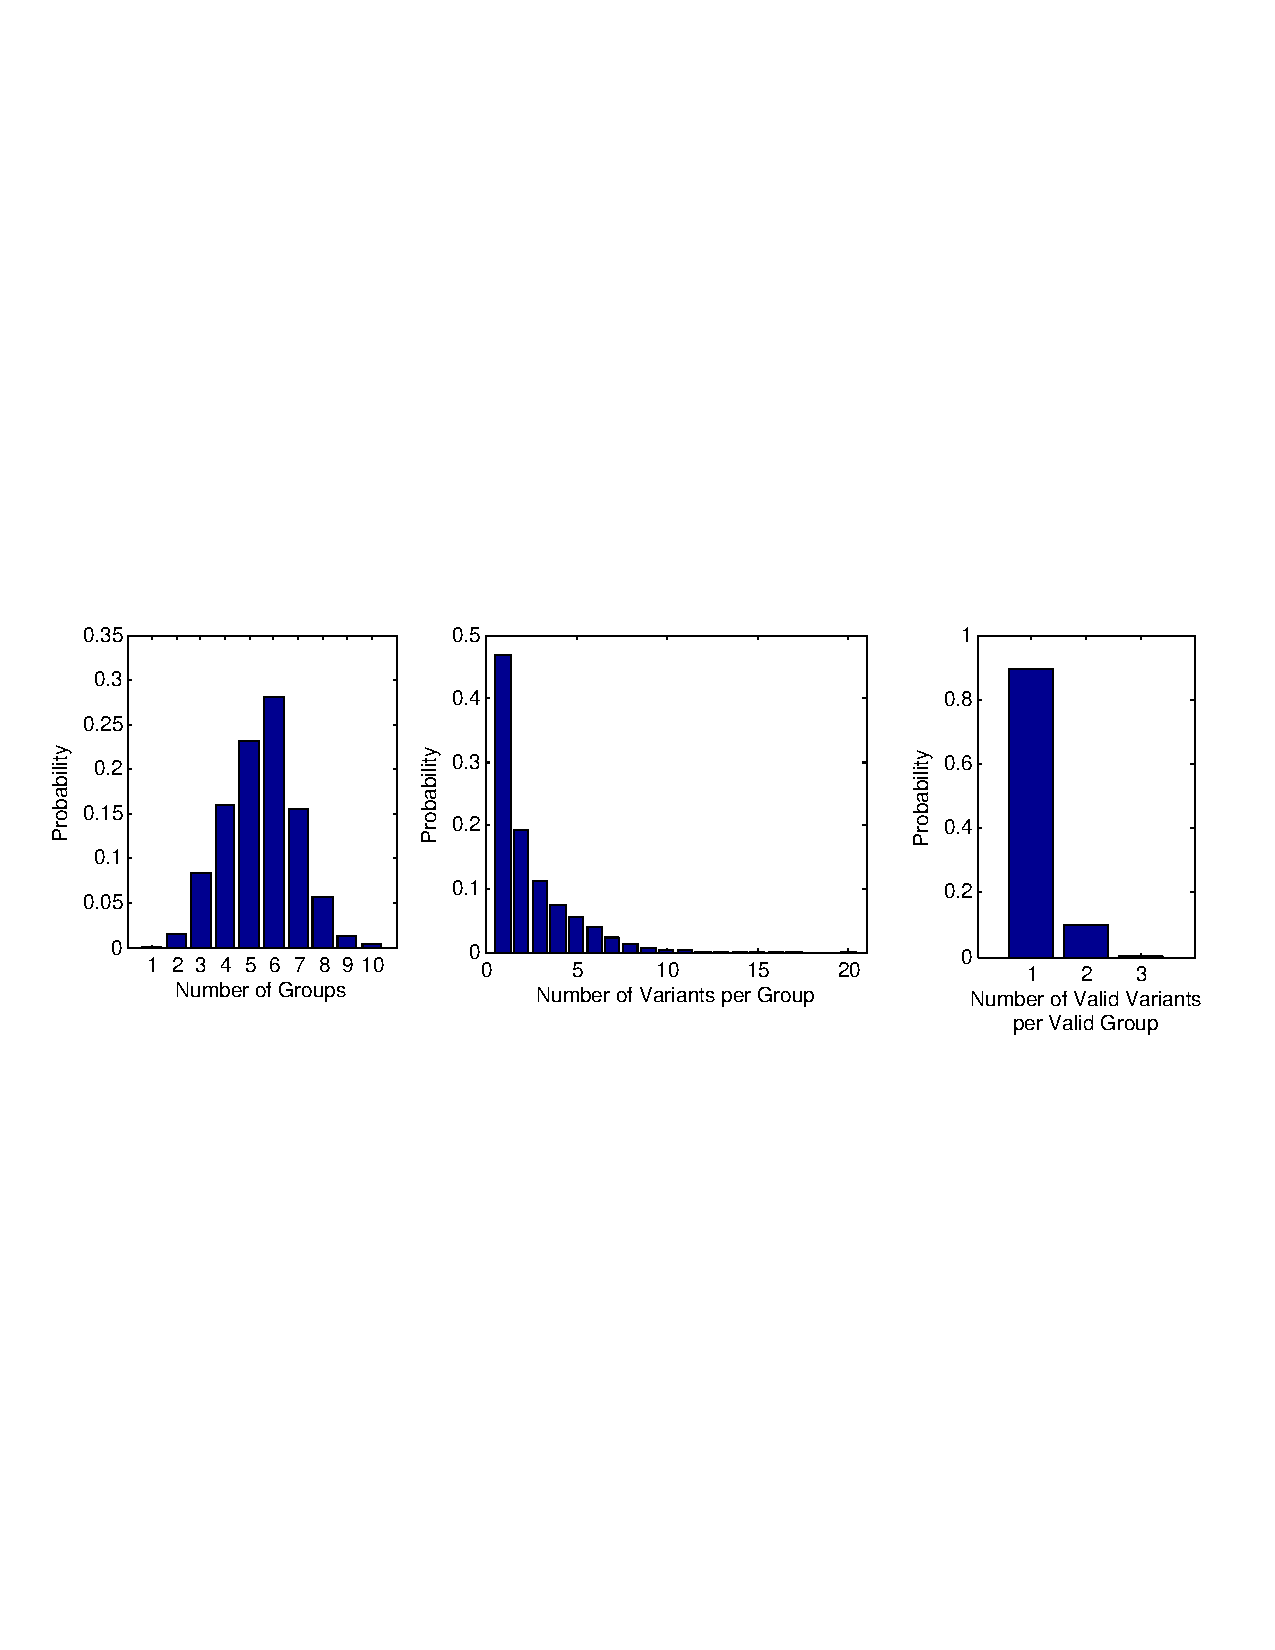
\includegraphics[trim = 4mm 90mm 4mm 90mm,clip,width=\textwidth]{fig/simulation/Simulation_hist_groups.pdf}
\caption[Variant group statistics for simulated data]{Distribution of (a) number of variant groups (b) size of variant groups (c) number of valid variants per valid group in the simulated data.}
\label{fig:Sim_hist_groups}
\end{figure}

We pool results from all of the datasets with mixtures of $k=1,2,3$ variants and evaluate our method on (1) identification (2) quantification of variant groups.

As described earlier, we are able to control FP rate on variant identification using target-decoy strategy. In Table~\ref{tbl:SimFDR}, we show the FDRs for a range of cutoffs on the estimated abundance of the variant groups. We also show the percentage of the cases with $k=1-4$ identified groups (estimated abundance $\ge$ cutoff) and the percentage of the cases with $k$ actual groups (actual abundance $\ge$ cutoff). In ideal sensitivity, the two percentages should be equal. As we see, the percentages inferred from the LP results closely follow the actual percentages. For example, at $1\%$ FDR (estimated abundance $\ge 20\%$) cutoff, we identify at least one variant group for $98.9\%$ of the cases; $1$ variant group in $51.0\%$, $2$ variant groups in $45.2\%$ and $3$ groups in $2.7\%$ of the cases. In the ideal case, we would identify exactly $1, 2$ and $3$ variant groups in $47.0\%, 47.6\%$ and $5.7\%$ of the cases, respectively. This result suggests that the sensitivity of our approach is close to the optimal.


% FDR results are similar to what we got in the lens dataset. FDR goes only up to $xxx\%$
% while the threshold for the estimated abundance can go as low as $xxx\%$. Also, even at a very low FDR rate, $xxx\%$, we are able to

\begin{table}[h]
  \centering
  \caption[Estimated FDRs of our approach on simulated data]{Estimated FDRs of our approach on simulated data for a range of cutoffs on the estimated abundance of the variant groups. At each FDR level, the percentage of the cases with $k = 1 - 4$ identified groups (estimated abundance $\ge$ cutoff) and (in parenthesis) the percentage of the cases with $k$ actual groups (actual abundance $\ge$ cutoff) are displayed.
  }\label{tbl:SimFDR}
\begin{tabular}{|c|l|l|l|l|l|l|}
\hline
Estimated Abundance & \multirow{2}{*}{FDR} & \multicolumn{5}{|c|}{\#Cases with k groups identified }\\
of Variant Group & & $k\ge 1$ & $k=1$ & $k=2$ & $k=3$ & $k=4$ \\
\hline
$\ge 60\%$ &0.002 &74.9\% (79.2\%) &74.9\% (79.2\%) &0.0\% (0.0\%) &0.0\% (0.0\%) &0.0\%\\
$\ge 55\%$ &0.002 &82.7\% (87.1\%) &82.7\% (87.1\%) &0.0\% (0.0\%) &0.0\% (0.0\%) &0.0\%\\
$\ge 50\%$ &0.003 &90.9\% (95.6\%) &90.8\% (95.6\%) &0.1\% (0.0\%) &0.0\% (0.0\%) &0.0\%\\
$\ge 45\%$ &0.003 &94.6\% (96.9\%) &89.6\% (89.1\%) &5.0\% (7.8\%) &0.0\% (0.0\%) &0.0\%\\
$\ge 40\%$ &0.003 &96.7\% (98.6\%) &84.5\% (83.2\%) &12.1\% (15.4\%) &0.0\% (0.0\%) &0.0\%\\
$\ge 35\%$ &0.004 &98.1\% (99.9\%) &77.7\% (75.7\%) &20.4\% (24.2\%) &0.0\% (0.0\%) &0.0\%\\
%$\ge 34\%$ &0.004 &98.3\% (100.0\%) &76.0\% (73.6\%) &22.3\% (26.4\%) &0.0\% (0.0\%) &0.0\%\\
%$\ge 32\%$ &0.005 &98.5\% (100.0\%) &72.6\% (69.7\%) &25.9\% (30.3\%) &0.0\% (0.0\%) &0.0\%\\
$\ge 30\%$ &0.005 &98.7\% (100.0\%) &68.8\% (65.5\%) &29.7\% (34.1\%) &0.1\% (0.3\%) &0.0\%\\
%$\ge 28\%$ &0.006 &98.8\% (100.0\%) &65.0\% (61.7\%) &33.4\% (37.5\%) &0.4\% (0.8\%) &0.0\%\\
%$\ge 26\%$ &0.007 &98.8\% (100.0\%) &61.1\% (57.8\%) &37.0\% (40.5\%) &0.8\% (1.7\%) &0.0\%\\
$\ge 25\%$ &0.007 &98.9\% (100.0\%) &59.2\% (55.9\%) &38.7\% (42.0\%) &1.0\% (2.1\%) &0.0\%\\
%$\ge 24\%$ &0.008 &98.9\% (100.0\%) &57.4\% (54.0\%) &40.2\% (43.3\%) &1.3\% (2.7\%) &0.0\%\\
%$\ge 23\%$ &0.008 &98.9\% (100.0\%) &55.7\% (52.2\%) &41.6\% (44.5\%) &1.6\% (3.3\%) &0.0\%\\
%$\ge 22\%$ &0.009 &98.9\% (100.0\%) &54.1\% (50.5\%) &42.8\% (45.5\%) &2.0\% (4.0\%) &0.0\%\\
%$\ge 21\%$ &0.010 &98.9\% (100.0\%) &52.5\% (48.7\%) &44.1\% (46.6\%) &2.3\% (4.6\%) &0.0\%\\
$\ge 20\%$ &0.010 &98.9\% (100.0\%) &51.0\% (47.0\%) &45.2\% (47.6\%) &2.7\% (5.4\%) &0.0\%\\
$\ge 15\%$ &0.019 &99.0\% (100.0\%) &48.7\% (47.0\%) &46.6\% (47.6\%) &3.7\% (5.4\%) &0.0\%\\
$\ge 10\%$ &0.036 &99.0\% (100.0\%) &47.9\% (47.0\%) &46.7\% (47.6\%) &4.4\% (5.4\%) &0.0\%\\
$\ge 5\%$ &0.077 &99.0\% (100.0\%) &47.6\% (47.0\%) &46.4\% (47.6\%) &4.9\% (5.4\%) &0.0\%\\
\hline
\end{tabular}
\end{table}

\clearpage
In order to measure the accuracy of the variant identifications, we calculate how often the variant groups identified are correct. We call a variant group identification \emph{correct}, if the group was initially assigned a non-zero abundance (i.e. $\ge$ min. abundance$=20\%$).
In Figure~\ref{fig:SimTopkCorrect}, we compare the percentage of the cases where we identify at least $k$ variant groups and the cases where \emph{top} (most abundant) $k$ identifications are correct at FDR $1\%$ for $k=1,2,3$. As shown in Figure~\ref{fig:SimTopkCorrect}a, when there is only one variant group present in the sample, we identify a single variant group in almost all ($99.3\%$) of the cases with very high accuracy ($99.9\%$). In Figure~\ref{fig:SimTopkCorrect}b,c the identification results on mixtures of $2$ and $3$ variant groups are shown. We achieve similarly very good performance in identification of both variant groups from a mixture of $2$ groups. We are able to correctly identify both groups in $90.0\%$ of the cases. In presence of $3$ variants, percentage of identification of all variants drops to $55.2\%$ but with $89.2\%$ accuracy.


%In presence of $3$ variant groups, top $1$ and $2$ identifications are correct in
%$94.2\%$ and $86.8\%$ of the cases, respectively. We identify $3$ variant groups in
%$55.2\%$ of the cases and in $89.2\%$ of those cases all the variants identified are correct.

%
%1 variant mixture
%>=k identified,  top k correct
%k=1    0.9929    0.9914
%k=2    0.0034         0
%k=3         0         0
%
%2 variants mixture
%>=k identified,  top k correct
%k=1    0.9932    0.9834
%k=2    0.9226    0.8990
%k=3    0.0176         0
%3 variants mixture
%>=k identified,  top k correct
%k=1    0.9638    0.9420
%k=2    0.9195    0.8681
%k=3    0.5515    0.4920
%
\begin{figure}[htbp]
\centering % trim=l b r t
a)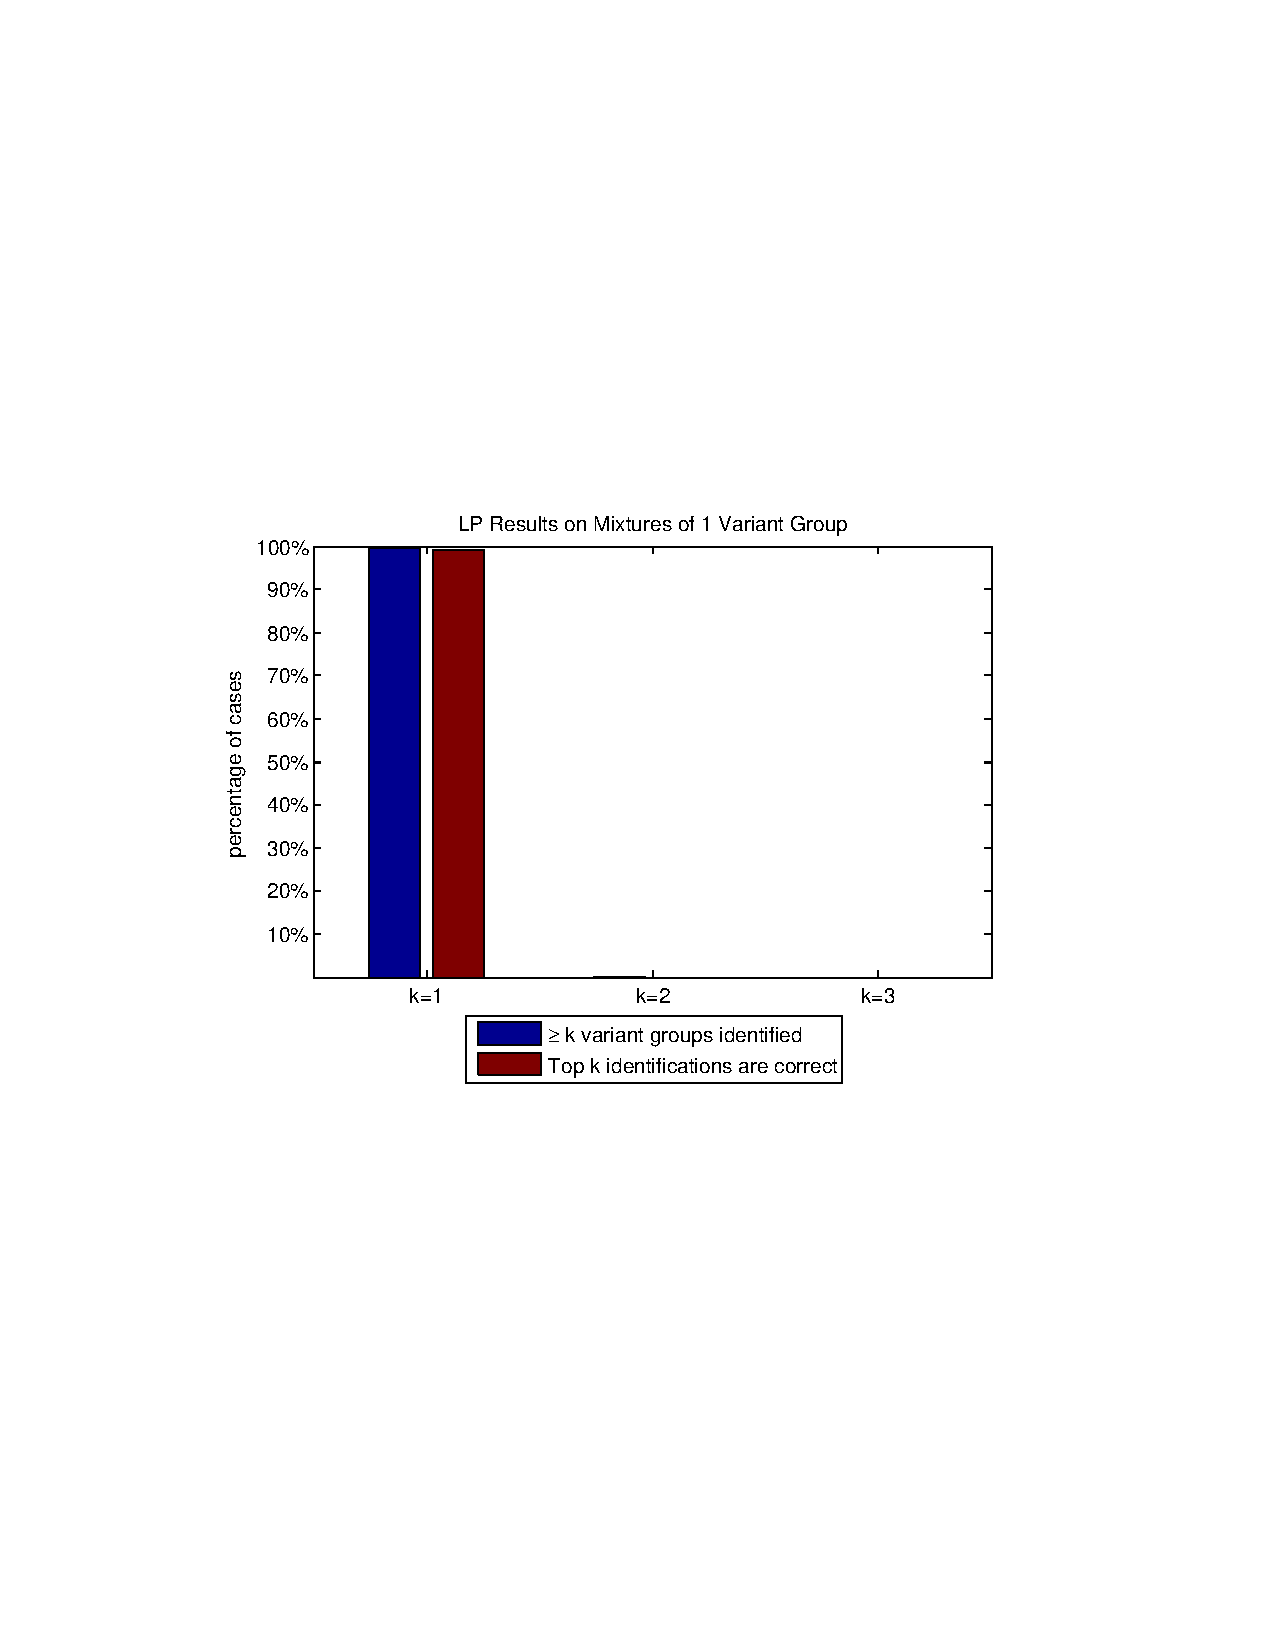
\includegraphics[trim = 30mm 80mm 40mm 80mm,clip, width=0.4\textwidth]{fig/simulation/topkcorrect_1variant.pdf}
b)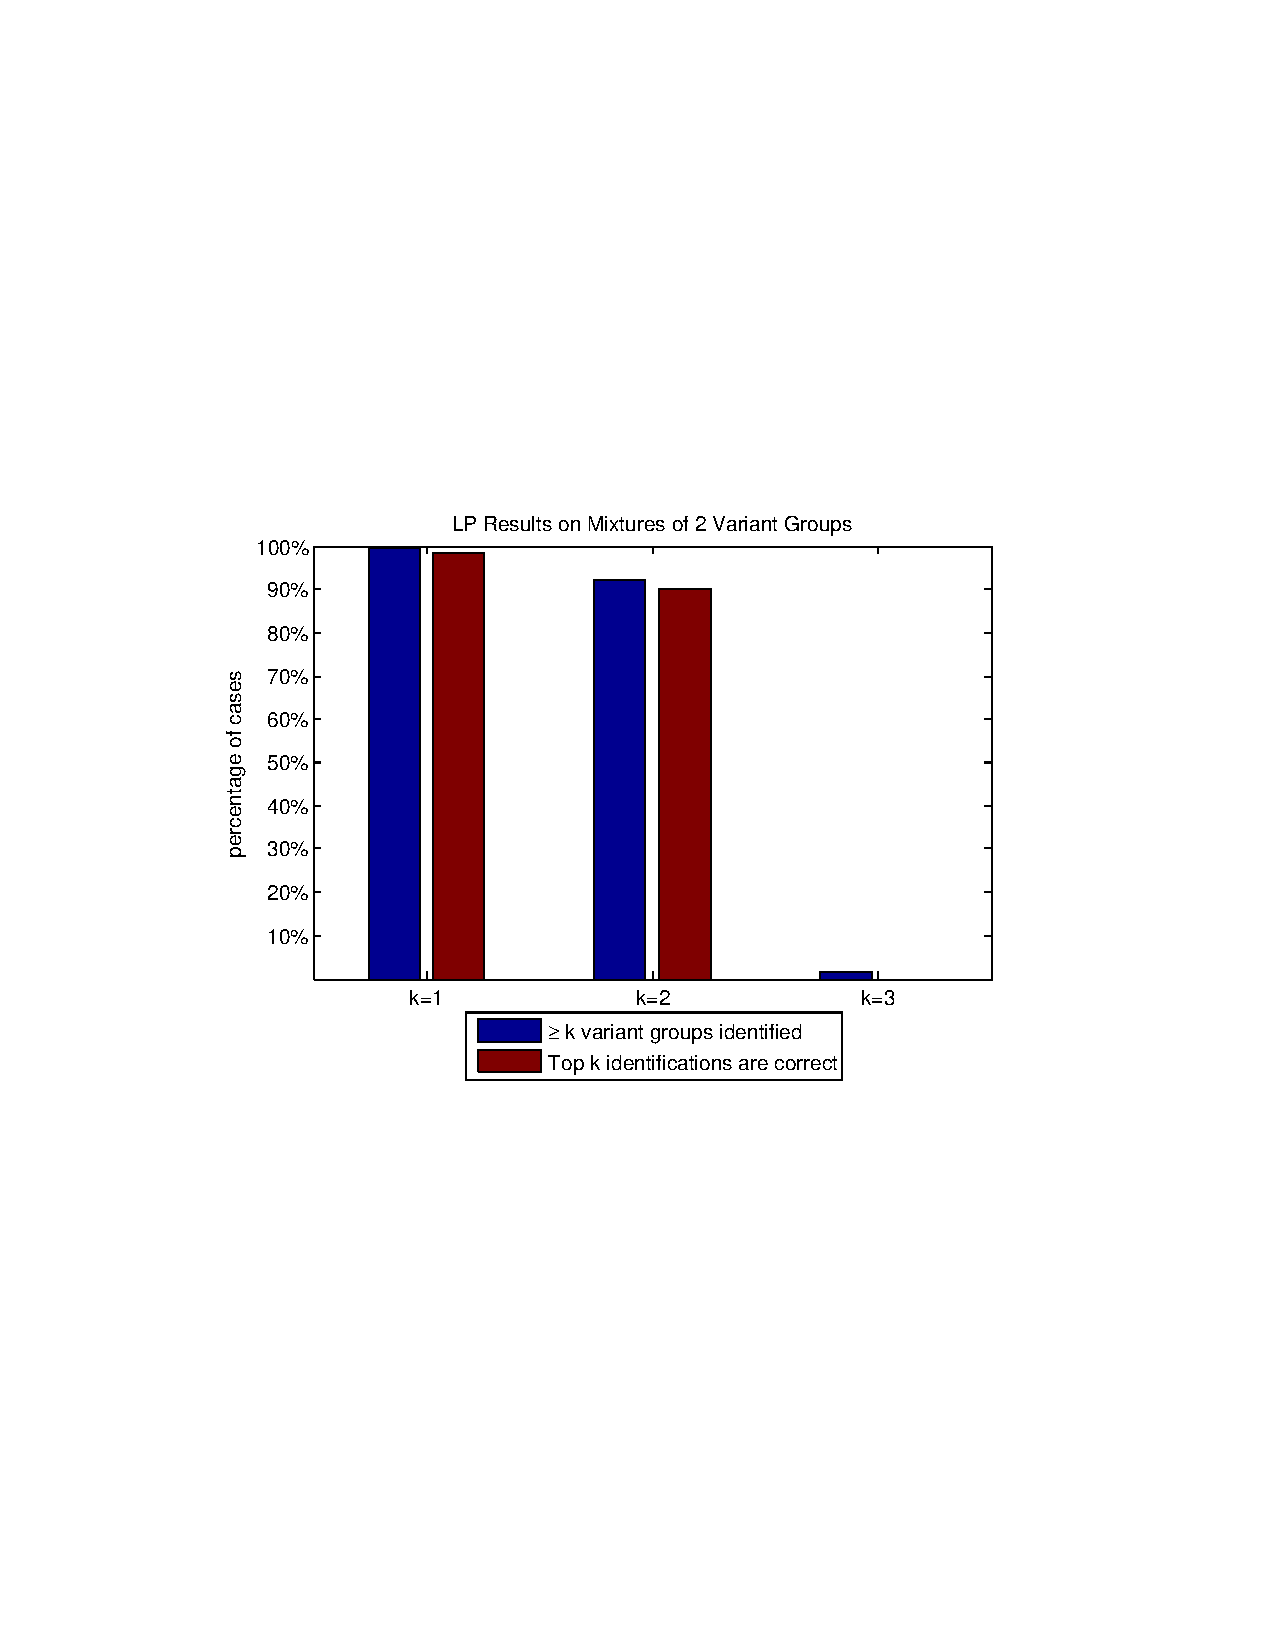
\includegraphics[trim = 30mm 80mm 40mm 80mm,clip, width=0.4\textwidth]{fig/simulation/topkcorrect_2variants.pdf}
c)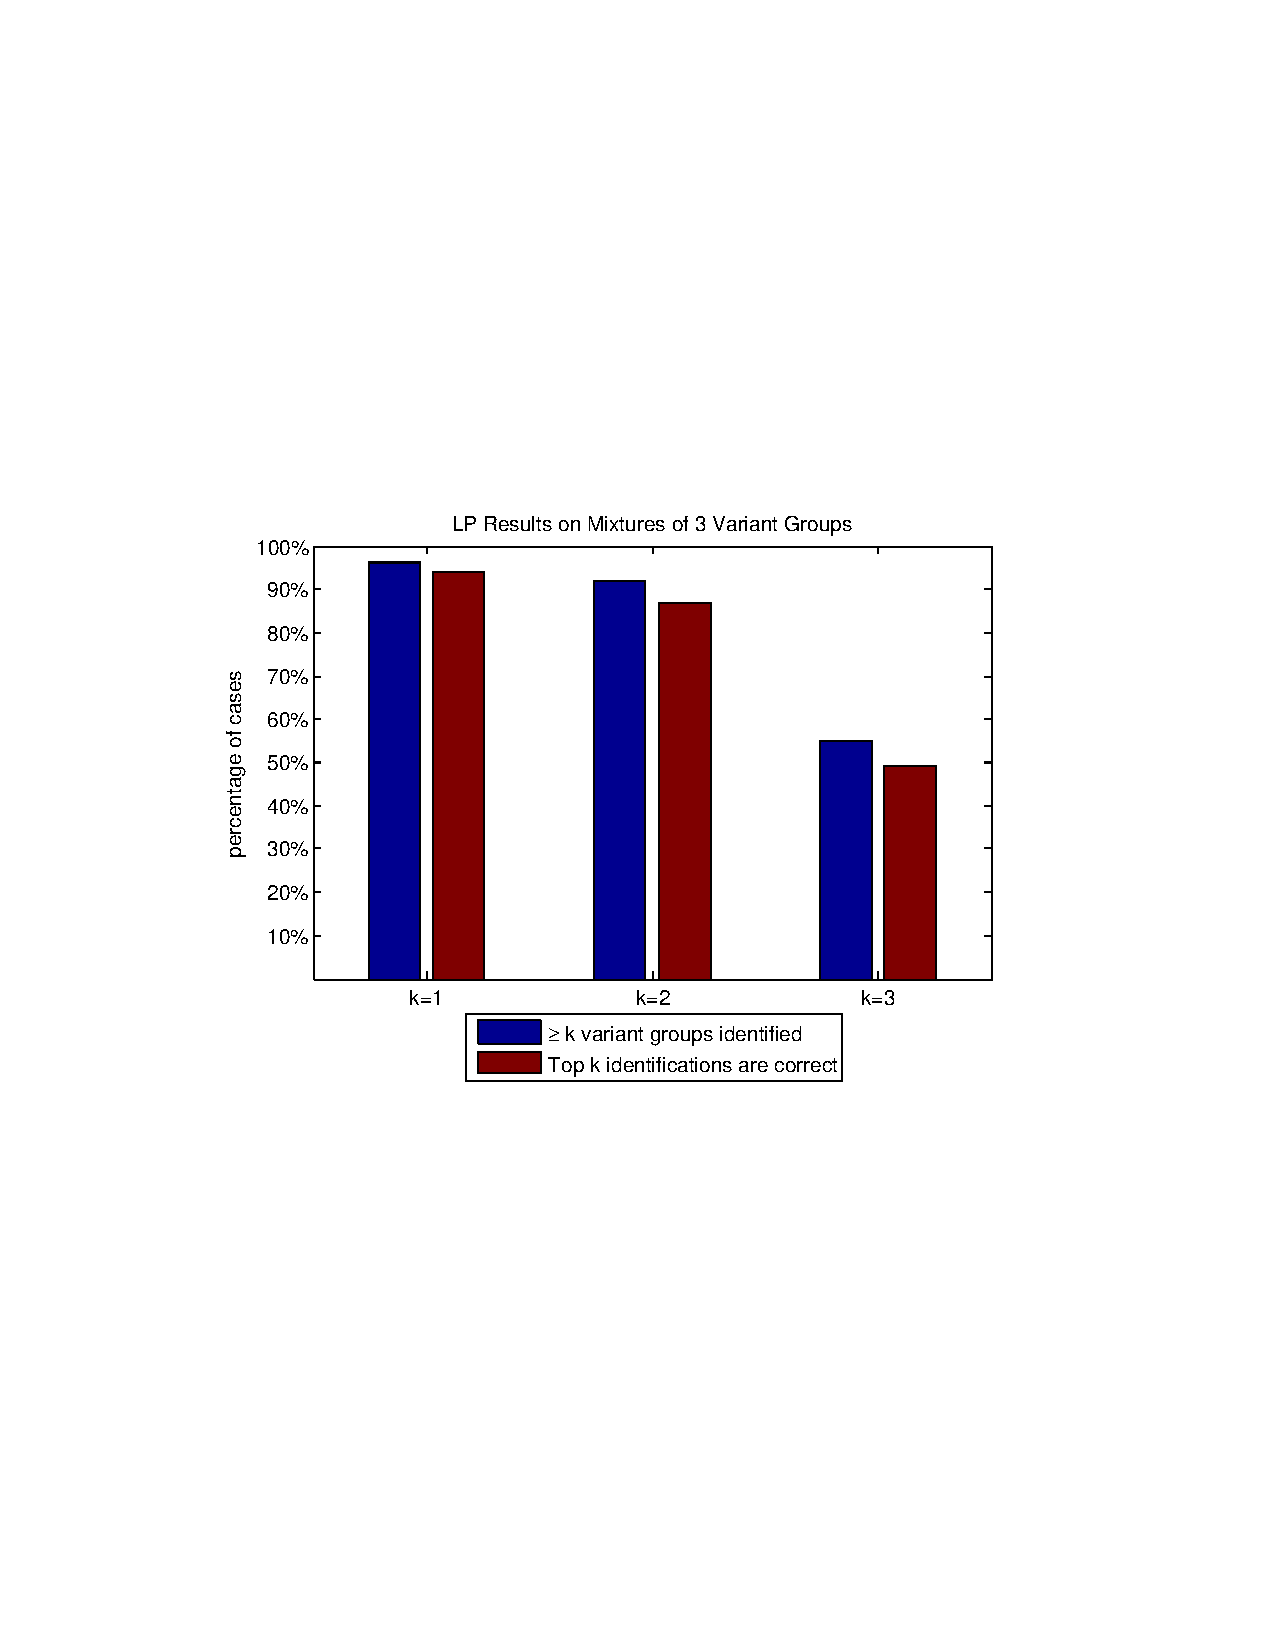
\includegraphics[trim = 30mm 80mm 40mm 80mm,clip, width=0.4\textwidth]{fig/simulation/topkcorrect_3variants.pdf}
\caption[Identification results on mixtures of $1$, $2$ and $3$ variant groups]{Identification results on mixtures of a) $1$, b) $2$ and c) $3$ variant groups at FDR=$1\%$. The  percentage of the cases where we identify at least $k$ variant groups and the cases where \emph{top} (most abundant) $k$ identifications are correct for $k=1,2,3$.}
\label{fig:SimTopkCorrect}
\end{figure}

We further investigate how the accuracy of the identifications change by the abundance of the variant groups. Figure~\ref{fig:SimTopkCorrect_byQ} demonstrate the percentage of $\geq k (1-3)$ identifications (white bars) and the correct top $k$ identifications (blue, green, red bars for $k$=$1$,$2$, and $3$, respectively) grouped by the abundance of actual most abundant variant group. As we can see, in the mixtures of $2$ variant groups, the percentage of the correct top $2$ identifications decreases from $95.9\%$ to $80.6\%$ while the percentage of correct top $1$ identification is almost the same ($>98\%$) suggesting that as the relative abundance of the $2$nd most abundant variant gets smaller, we are more likely not to identify the $2nd$ variant group. Note that the accuracy is still more than $90\%$ for the correct $2$nd variant group identification. Similarly, in the mixtures of $3$ variant groups, as the relative abundances of the $2$nd and $3$rd most abundant variants gets smaller, the percentage of the identifications of $2$ or more groups decreases from $92.1\%$ to $88.9\%$ and of $3$ variants from $60\%$ to $43.5$. However, in all those cases, accuracy is above $85\%$.

%2 variants mixture, >=k identified
%Q = 50-60, 60-70, 70-80\%
%k=1    0.9917    0.9937    0.9942
%k=2    0.9829    0.9605    0.8300
%k=3    0.0248    0.0155    0.0128
%3 variants mixture, >=k identified
%Q = 30-40, 40-50, 50-60
%k=1    0.9569    0.9665    0.9652
%k=2    0.9214    0.9282    0.8891
%k=3    0.6055    0.5643    0.4348
%
%2 variants mixture, top k correct
%Q = 50-60, 60-70, 70-80\%
%k=1    0.9820    0.9838    0.9844
%k=2    0.9590    0.9376    0.8061
%k=3         0         0         0
%3 variants mixture, top k correct
%Q = 30-40, 40-50, 50-60
%k=1    0.9414    0.9494    0.9196
%k=2    0.8737    0.8776    0.8304
%k=3    0.5393    0.5096    0.3696
%
\begin{figure}[htbp]
\centering % trim=l b r t
a)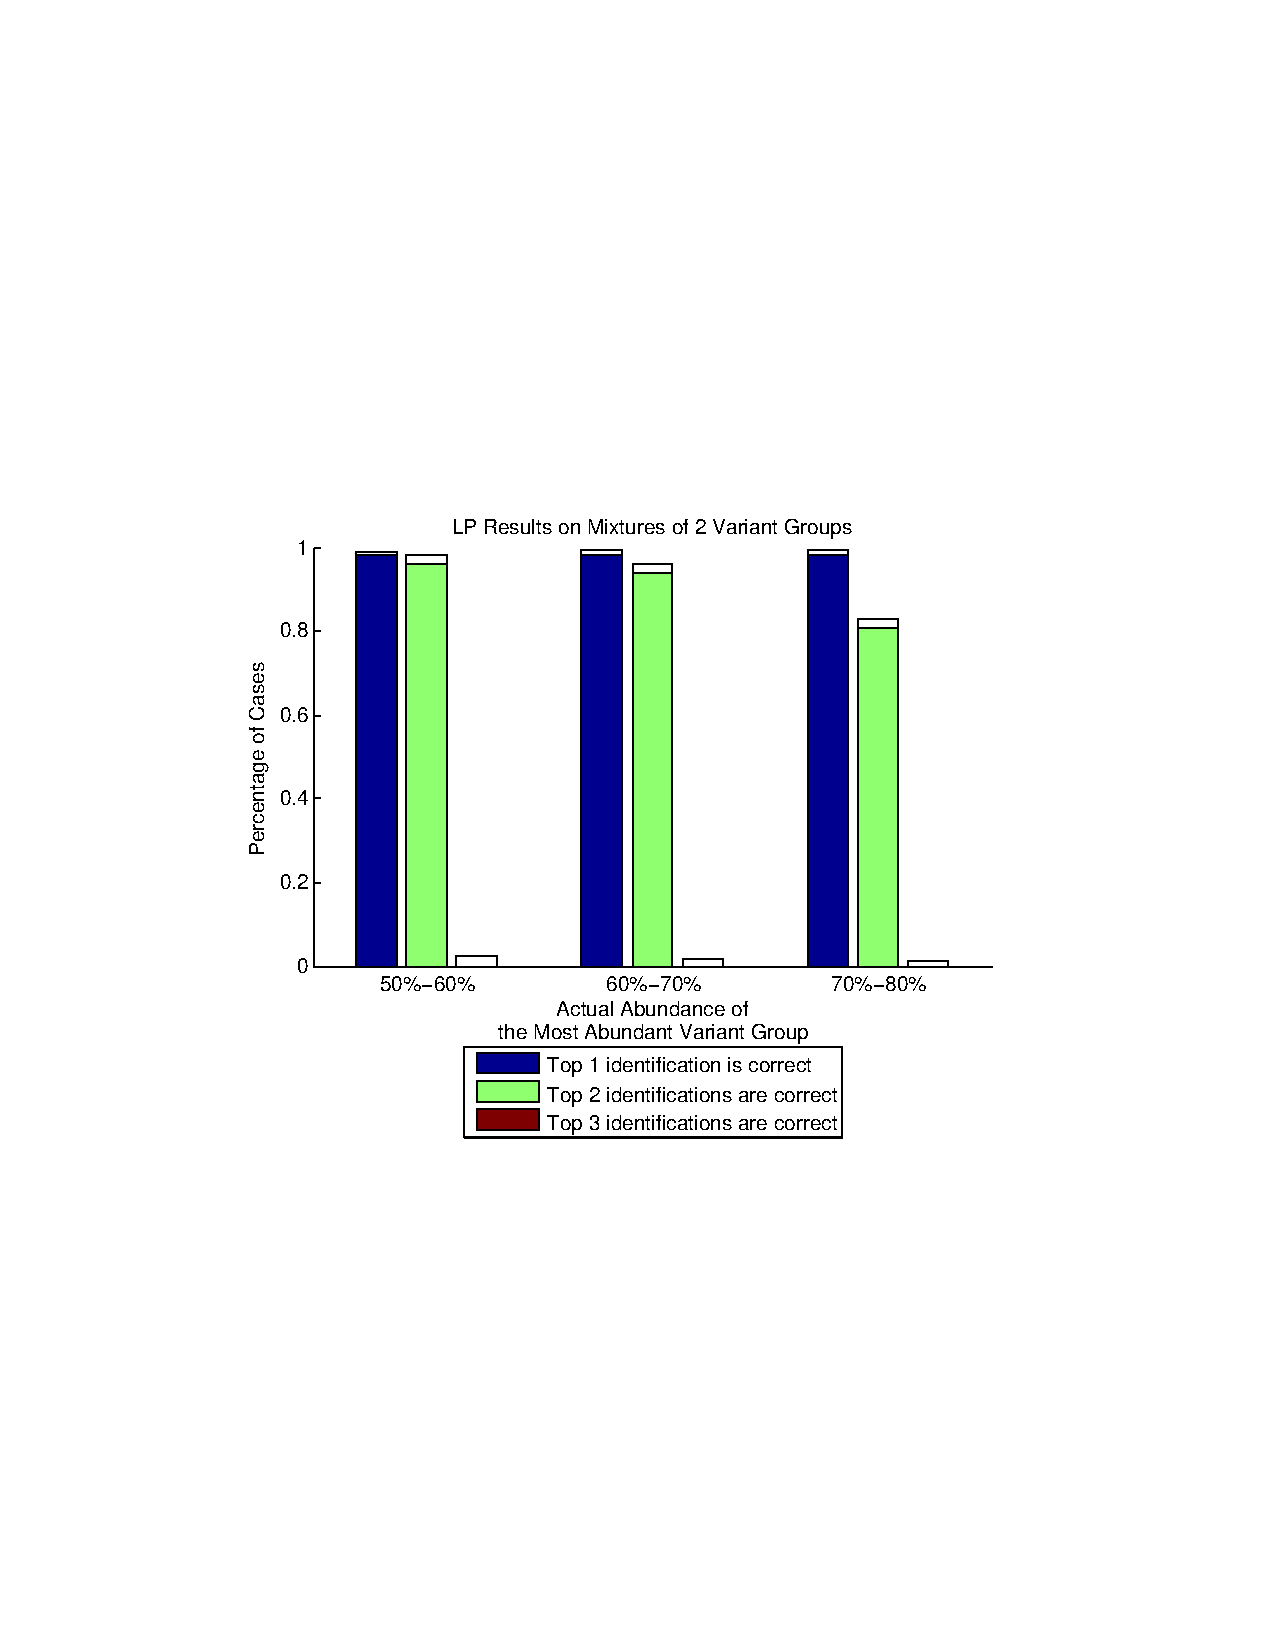
\includegraphics[trim = 30mm 80mm 40mm 80mm,clip, width=0.5\textwidth]{fig/simulation/topkcorrect_2variants_byQ.pdf}
b)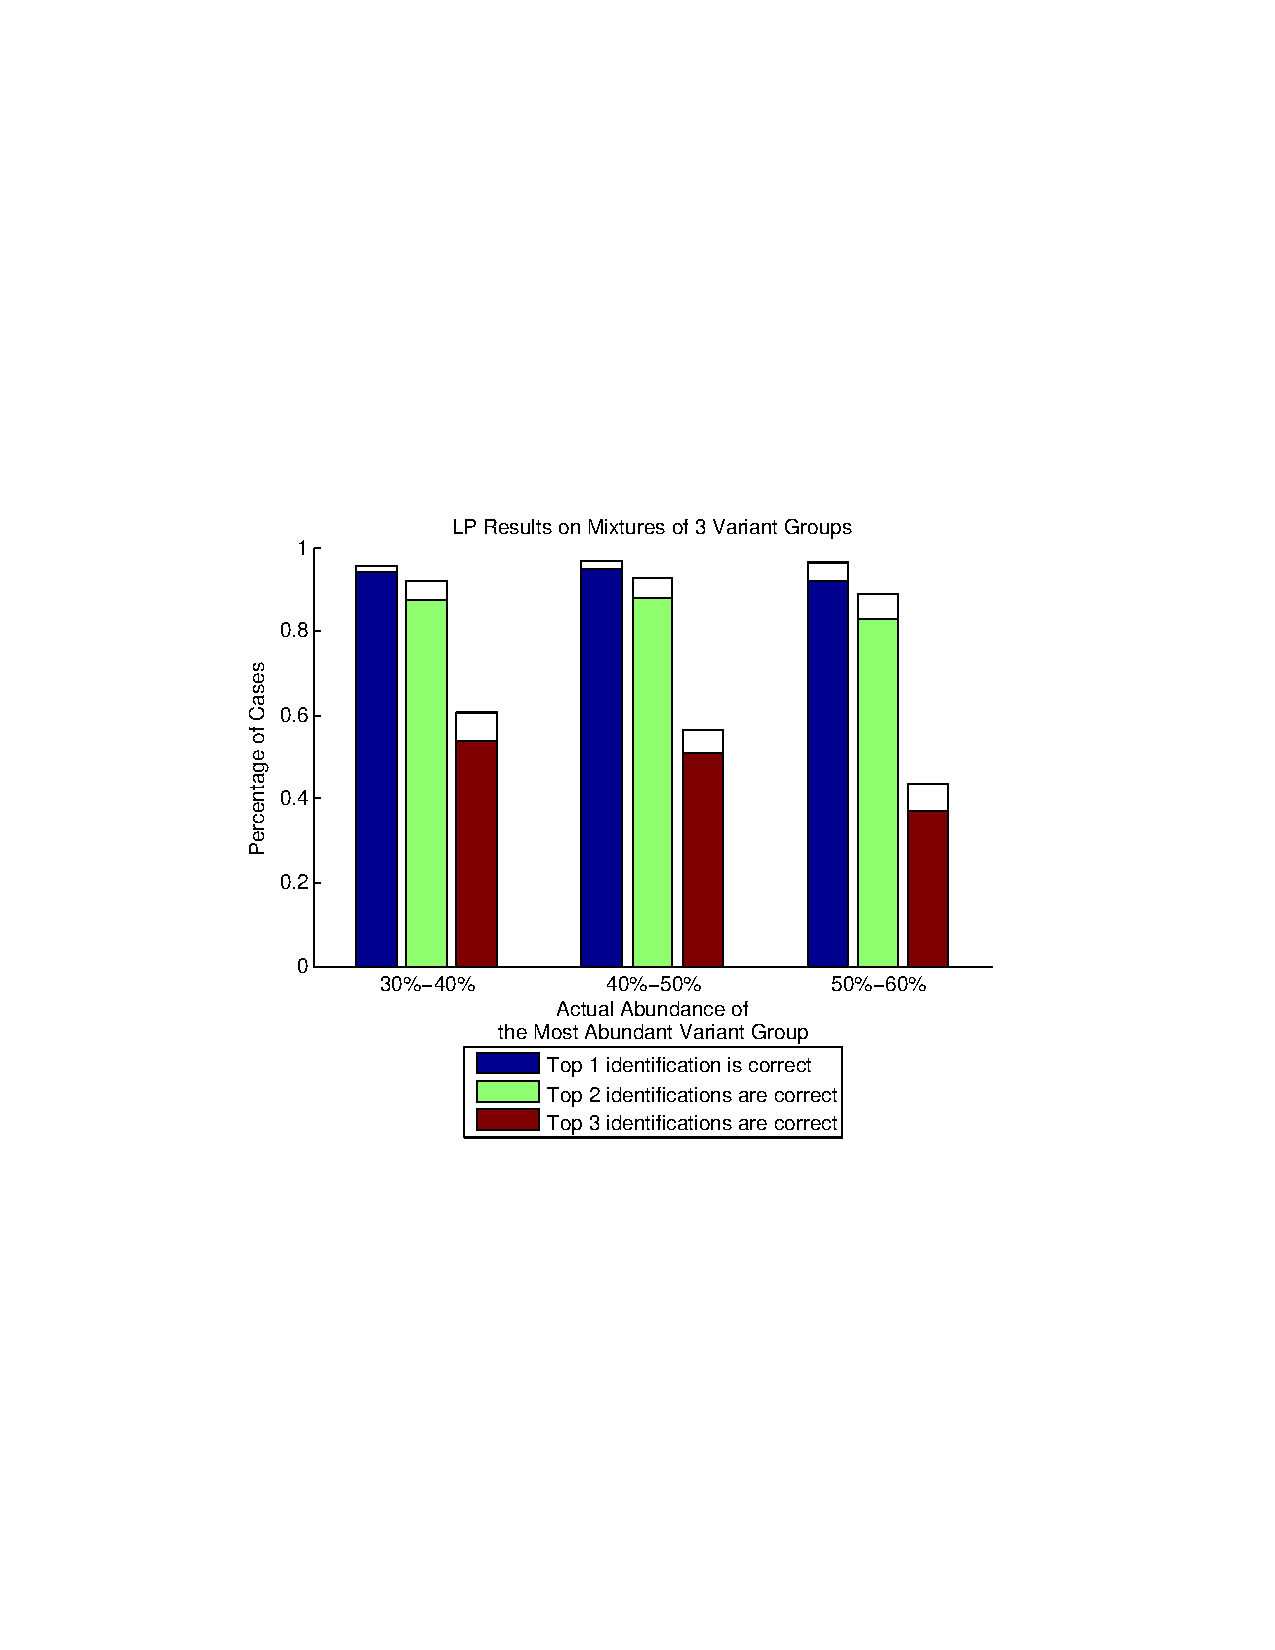
\includegraphics[trim = 30mm 80mm 40mm 80mm,clip, width=0.5\textwidth]{fig/simulation/topkcorrect_3variants_byQ.pdf}
\caption[Identification results on mixtures of $2$ and $3$ variant groups]{Identification results on mixtures of a) $2$ and b) $3$ variant groups at FDR=$1\%$. Colored bars show the percentage of the cases where \emph{top} (most abundant) $k$ ($1-3$) identifications are correct grouped by the actual abundance of the most abundant the variant group. Non-colored (white) bars indicate the percentage of the cases with $\geq k$ group identifications.}
\label{fig:SimTopkCorrect_byQ}
\end{figure}

Besides identification of the present variants, our approach also reports relative abundances of the identified variant groups. We evaluate our quantification results by comparing the estimated and actual abundance of the identified variant groups in mixtures of $2$ and $3$ groups. The boxplots of log ratios of the estimated abundances of identified variant groups to their actual abundances, shown in Figure~\ref{fig:SimActualvsEstBoxPlot}ab, are constructed with $5$, $25$, $50$, $75$, and $95$ percentiles. We observe that $90\%$ of the variant groups are accurately quantified with less than $0.5$ and $1$ fold difference of their actual abundance in mixtures of $2$ and $3$ variant groups, respectively.

\begin{figure}[htbp]
\centering % trim=l b r t
a)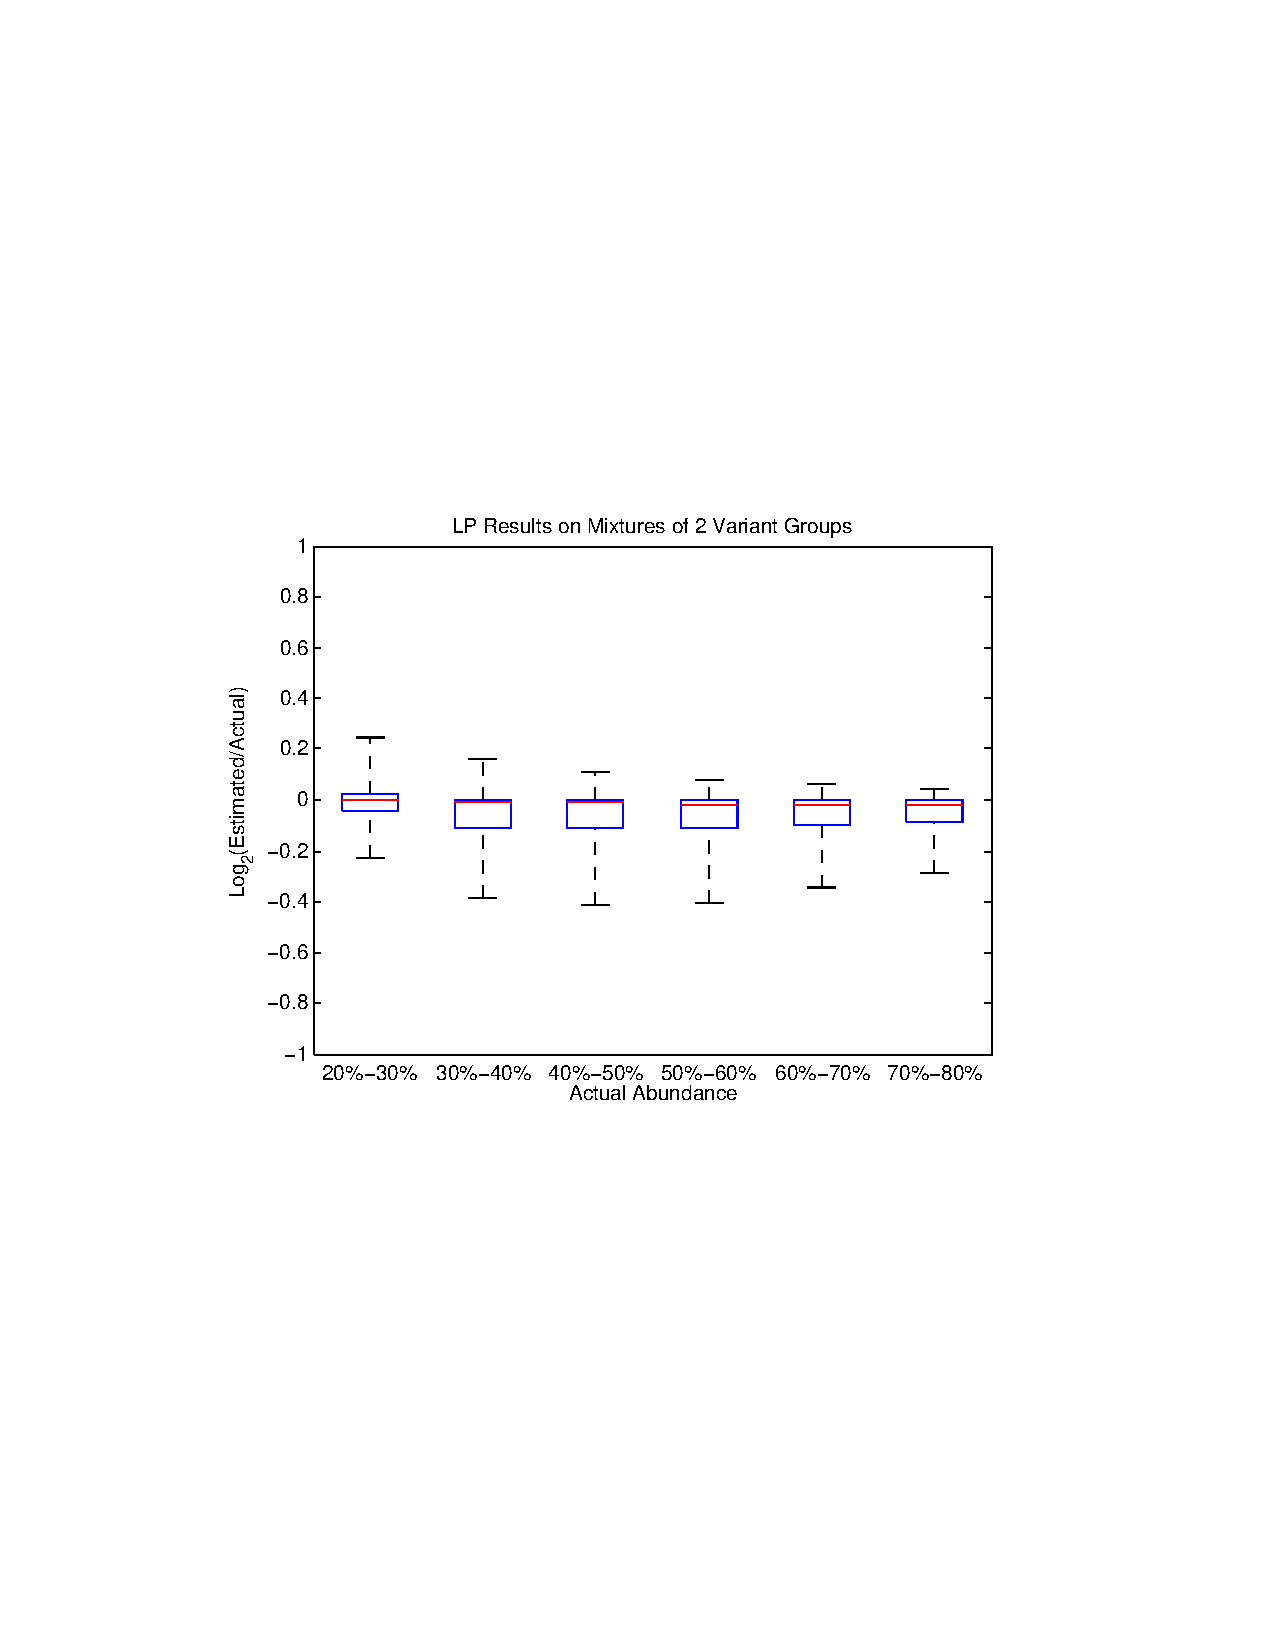
\includegraphics[trim = 30mm 80mm 40mm 80mm,clip, width=0.45\textwidth]{fig/simulation/boxplot_actualvsEst_2variants.pdf}
b)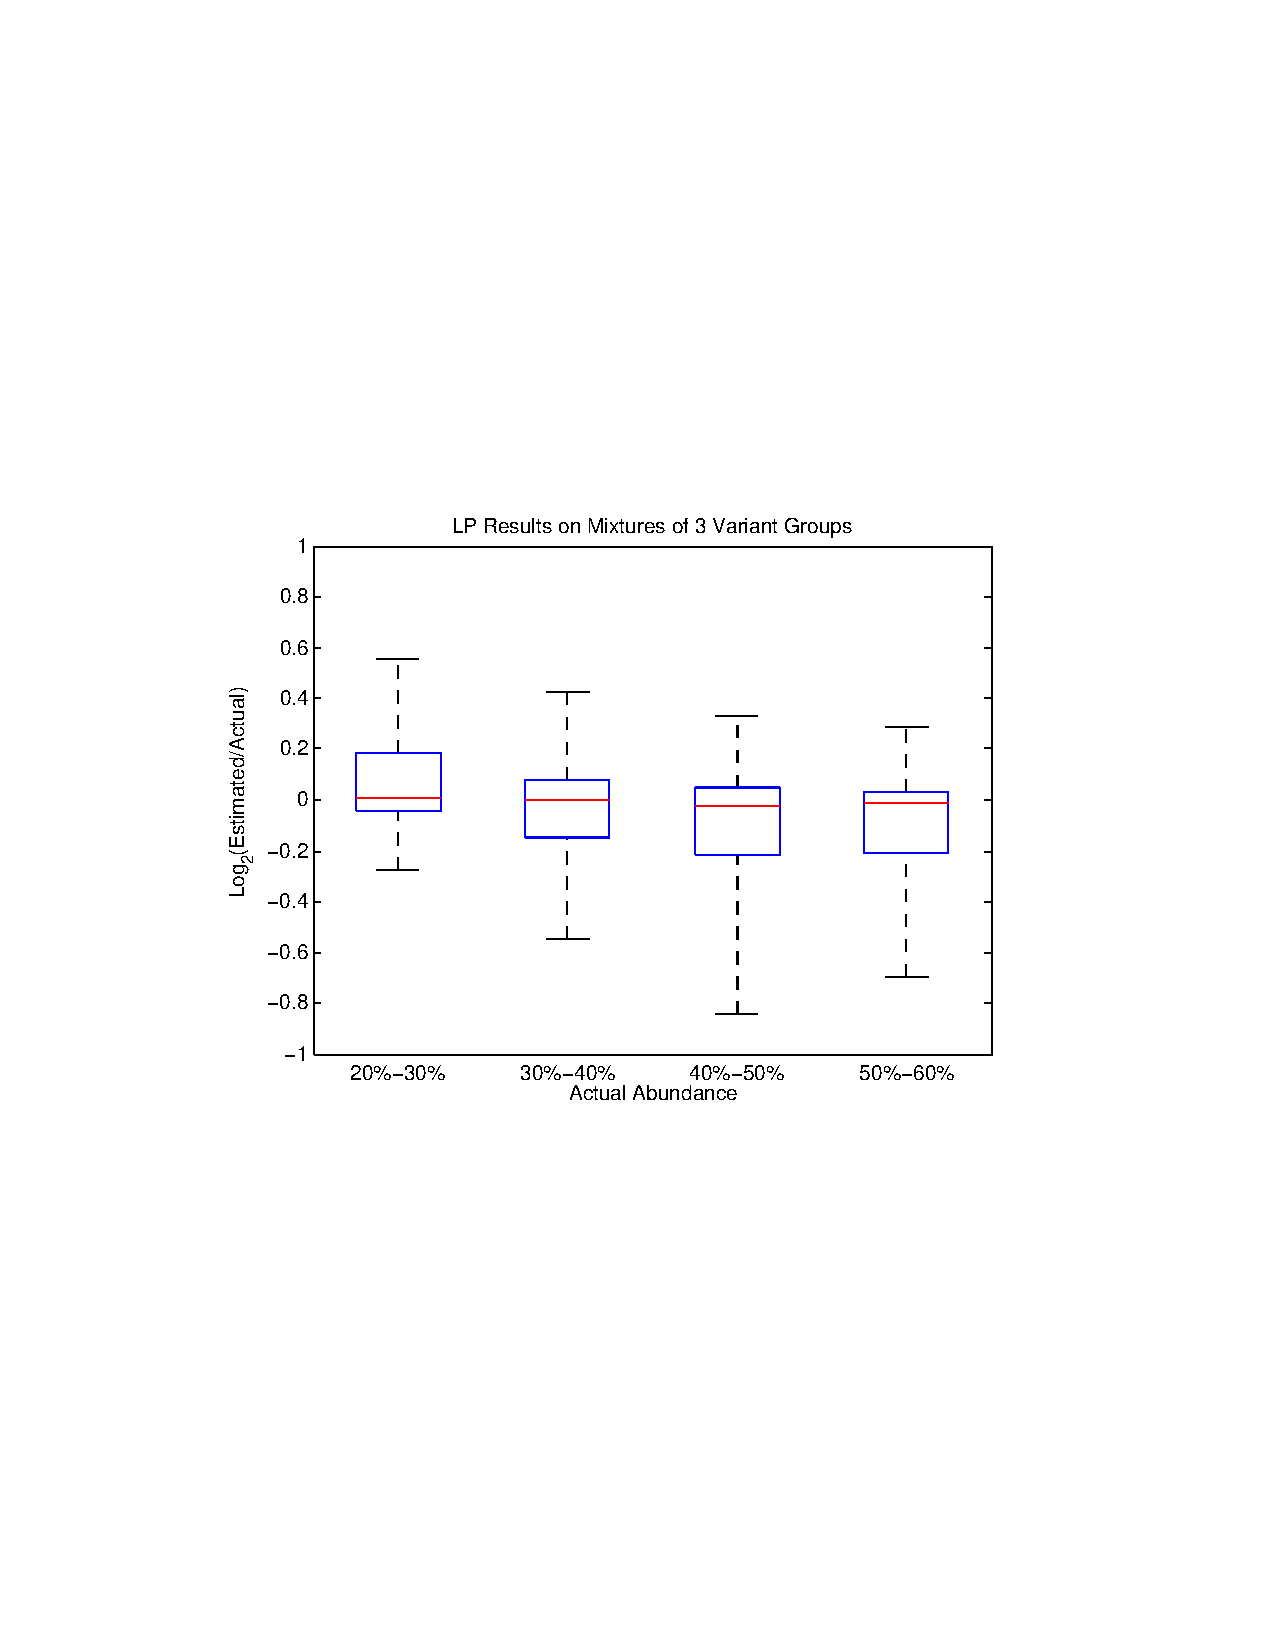
\includegraphics[trim = 30mm 80mm 40mm 80mm,clip, width=0.45\textwidth]{fig/simulation/boxplot_actualvsEst_3variants.pdf}
\caption[Quantification results on mixtures of $2$ and $3$ variant groups]{Quantification results on mixtures of a) $2$ and b) $3$ variant groups at FDR=$1\%$.
Box plot displays the distribution of the log ratio of the estimated abundance to the actual abundance of the variant groups. The bottom and top of the box are the $25$th and $75$th percentile (the lower and upper quartiles, respectively), and the band near the middle of the box is the $50$th percentile (the median). The ends of the whiskers represent the $5$th and $95$th percentiles.}
\label{fig:SimActualvsEstBoxPlot}
\end{figure}
